\section{Implementation}

The method of using a shunt resistor was chosen to measure the energy consumption because of its simple design which lets the student threat the system as a black box. The other measurment and estimation techniques where either too complex or didnt have a low enough error rate. Figure \ref{fig:deploy} shows the deployment diagram of the rig that is used to measure the energy consumption of the GPS reciever. 

\begin{figure}[H]
\centering
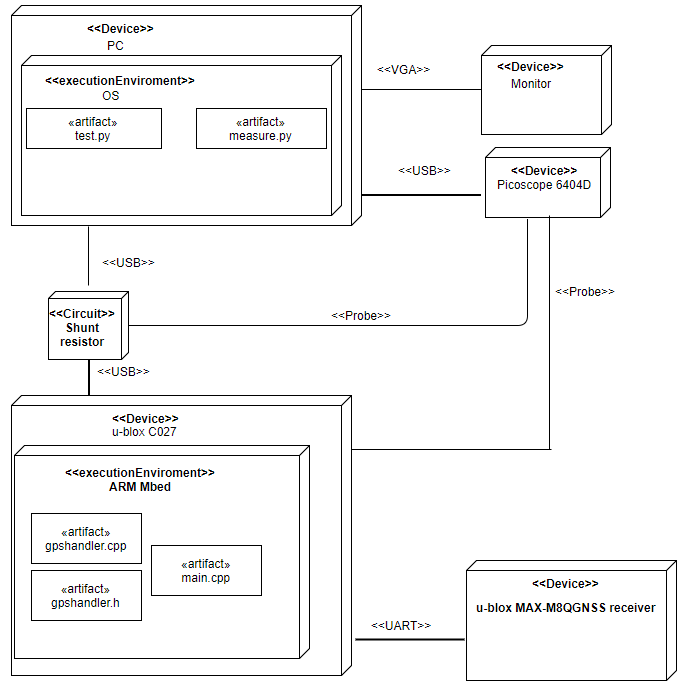
\includegraphics[height=4.5cm]{Project_Report/Images/deploy.PNG}
\caption{The deployment diagram for the rig that is used for measuring the energy consumption}
\label{fig:deploy}
\end{figure}

The measurement setup consist of the LoPy microcontroller along with the Pytrack from Pycom, the Picoscope 640AD from picotech, a shunt resistor, and a laptop. The platform is mounted inside a box on a cycle wagon to make the platform mobile. The following section will explain the role of each part in platform.

\subsection{LoPy}
\subsection{Shunt resistor}
\subsection{PC}
\subsection{Picoscope 640 AD}


\newpage